\documentclass[twocolumn,letterpaper]{scrartcl}

%%% Uncomment the following 2 lines if you want line numbers
\usepackage[switch]{lineno}
\linenumbers

\usepackage[english]{babel}
\usepackage{blindtext}
%\usepackage[margin=0.75in]{geometry}
\usepackage[sorting=none, maxbibnames=99]{biblatex}
\usepackage[breaklinks=true, colorlinks=True, allcolors=blue]{hyperref}
\usepackage{graphicx}
\usepackage[font={small}]{caption}
\addbibresource{CRB.bib} 
\usepackage{todonotes}
%\usepackage{float}

% The following lines add color to title, section, and subsection headings.
% Matches color used for FIDLs.
\usepackage{xcolor}
\definecolor{FIDL}{RGB}{31,98,66}
\addtokomafont{title}{\color{FIDL}}
\addtokomafont{section}{\color{FIDL}}
\addtokomafont{subsection}{\color{FIDL}}

\begin{document}

%\titlehead{Forest Insect \& Disease Leaflet}	
\title{DRAFT 2: Coconut Rhinoceros Beetle FIDL}
\author{Aubrey Moore, Trevor Jackson, Roland Quitugua\\ Robert Bevacqua, Jonae Sayama, and Ross Miller}
\maketitle

%%% Uncomment the following line if you want a table of comments
%\tableofcontents

\newpage

\begin{figure}[h]
	\centering
	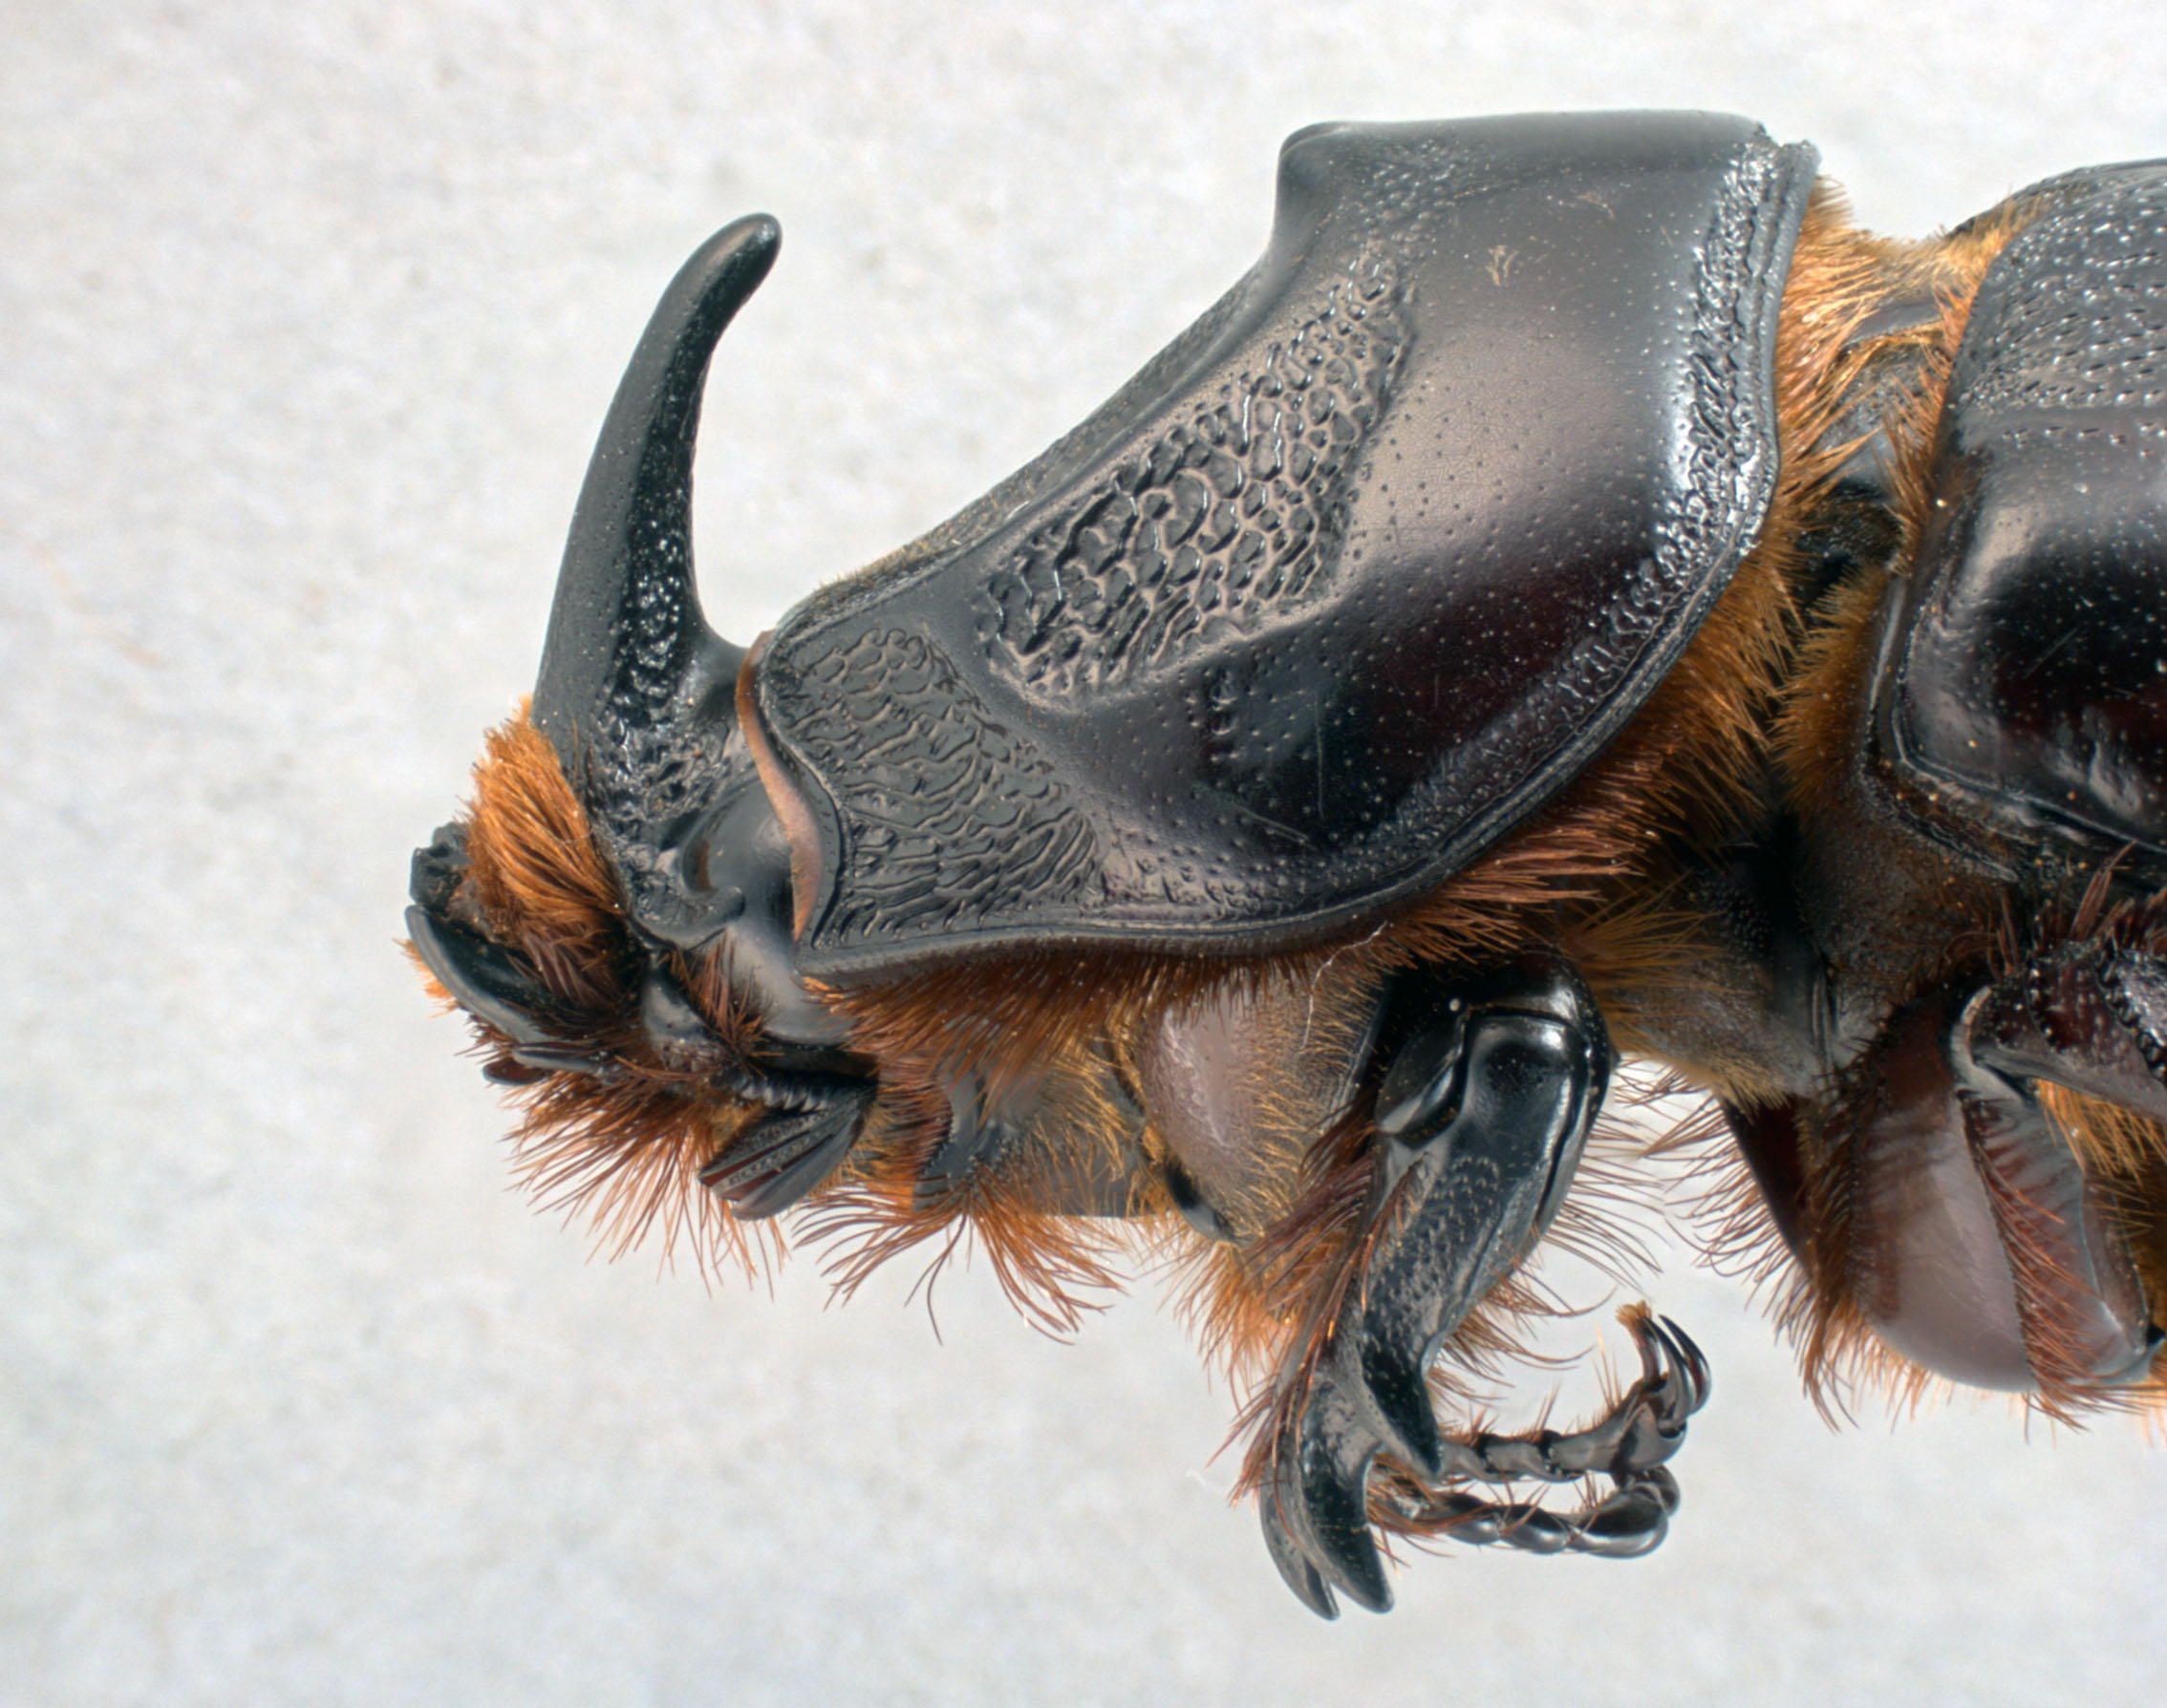
\includegraphics[width=\linewidth]{images/rhino_beetle_head}
	\caption{Male coconut rhinoceros beetle head and pronotum.}
	\label{fig:rhinobeetlehead}
\end{figure}

Coconut rhinoceros beetle (CRB) (Fig. \ref{fig:rhinobeetlehead}), \textit{Oryctes rhinoceros} (L.) (Coleoptera: Scarabaeidae) is a major pest of coconut palm and oil palm. It is native to southeast Asia, but it has invaded many Pacific islands. American affiliated islands invaded by CRB include American Samoa, the Republic of Palau, Guam, Oahu (Hawaii), and Rota (Commonwealth of the Northern Mariana Islands). With the exception of American Samoa, these islands have recently been invaded by a newly discovered variant of CRB referred as the CRB-G biotype. This highly invasive biotype is problematic because it is resistant to \textit{Oryctes rhinoceros} nudivirus OrNV, a classical biological control agent which previously controlled CRB on Pacific Islands. Throughout this leaflet, CRB-G refers to the virus-resistant biotype and CRB-S refers to virus-susceptible biotypes which can be readily controlled by OrNV.

\section{Biology}

\subsection{Taxonomy}

The coconut rhinoceros beetle (CRB), \textit{Oryctes rhinoceros} L., is a member of the scarab beetle  family, Scarabaeidae, and the subfamily Dynastinae. Taxonomic expertise is required to differentiate \textit{O. rhinoceros} from several other similar \textit{Oryctes} species, some of which also attack coconut and other palms.


\subsection{Life cycle and reproduction}
CRB has four life stages: eggs, grubs, pupae and adults with the grubs having three substages called instars (Fig. \ref{fig:crblifecycle}). The life span depends on environmental conditions, varying between 9 months and 18 months. Generation time varies between 5 months and 9 months.
The CRB sex ratio is usually close to 50:50 and females lay about 65 eggs during their lifetime. Under optimal environmental conditions with an unlimited food supply, CRB populations have the potential to grow at a rate of 3,250\% per generation.

\begin{figure}[h!]
	\centering
	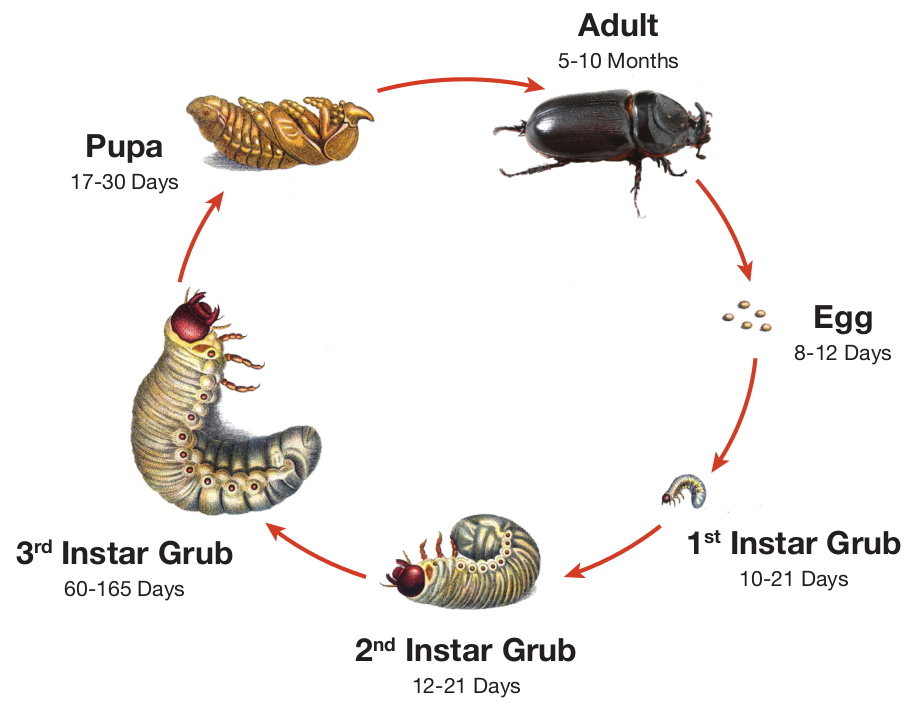
\includegraphics[width=\linewidth]{images/crb_life_cycle}
	\caption{Coconut rhinoceros beetle life cycle.}
	\label{fig:crblifecycle}
\end{figure}

\subsection{Larval feeding behavior}

Grubs feed only on decaying vegetation and do no harm. They feed in breeding sites which can be composed of a wide variety decaying vegetation. Preferred sites are standing dead coconut stems and fallen coconut logs and fronds. But breeding sites can be found in piles of a wide variety of organic material including green waste, dead trees of any species, saw dust, and manure. CRB breeding sites have even been found in commercially bagged soil purchased from  hardware stores. Active breeding sites contain all CRB life stages.

It is interesting to note that CRB individuals are at their heaviest during the prepupal stage (third instar grubs which have finished feeding). Thus almost all the biomass in a CRB population comes from conversion of decaying vegetation consumed during the larval stage and not from live plant material.

\subsection{Adult feeding behavior and damage symptoms}

CRB causes damage only in the adult stage. Both sexes feed on sap released from mascerated soft tissues within stems of several tropical monocot plants. Primary host plants are coconut palm and oil palm, but they also attack many other palm species.  Occasionally, they will attack other monocots such as banana, sago, pandanus, taro, pineapple, sugarcane, papaya and agave. However, CRB is not reported to be a major economic pest of these secondary hosts.

In both coconut palm and oil palm, CRB adults fly into the crown and force their way down between the leaf axils until they find a position where they can bore a horizontal hole into the crownshaft towards the white tissue at the center of the stem. When boring this hole, they will pass through one or more developing fronds. When these damaged fronds emerge from the crownshaft several weeks later, the damage will become evident as v-shaped cuts which are a distinctive sign of CRB damage (Fig. \ref{fig:dyingcoconuts} and \ref{fig:vshaped-cuts}). Occasionally, similar damage will appear in palms that have been trimmed to prevent contact with power lines or to remove nuts. However, in these cases, there will be no bore holes associated with the damage. If CRB caused a v-shaped cut, this can always be confirmed by removing outer petioles until a bore hole is found (Fig. \ref{fig:bore-hole-through-petiole} and \ref{fig:bore-hole}).

Adults feed for only a few days in the crown before exiting the bore hole to fly off to a breeding site for mating and oviposition. Adults feed every few weeks during their adult lifespan. Thus a single adult can damage several trees.

The impact of v-shaped cuts reduces production of nuts and degrades the aesthetic appeal of ornamental palms. However, the damage is not necessarily permanent. Even severely damaged palms can be nursed back to full health if all further attacks from adults are prevented.

CRB can cause palm mortality if a bore hole damages the single meristem (growing tip) within the base of the crownshaft. Mature palm mortality caused by CRB is rare unless the adult population and the associated attack rate is very high.   

\begin{figure}[h]
	\centering
	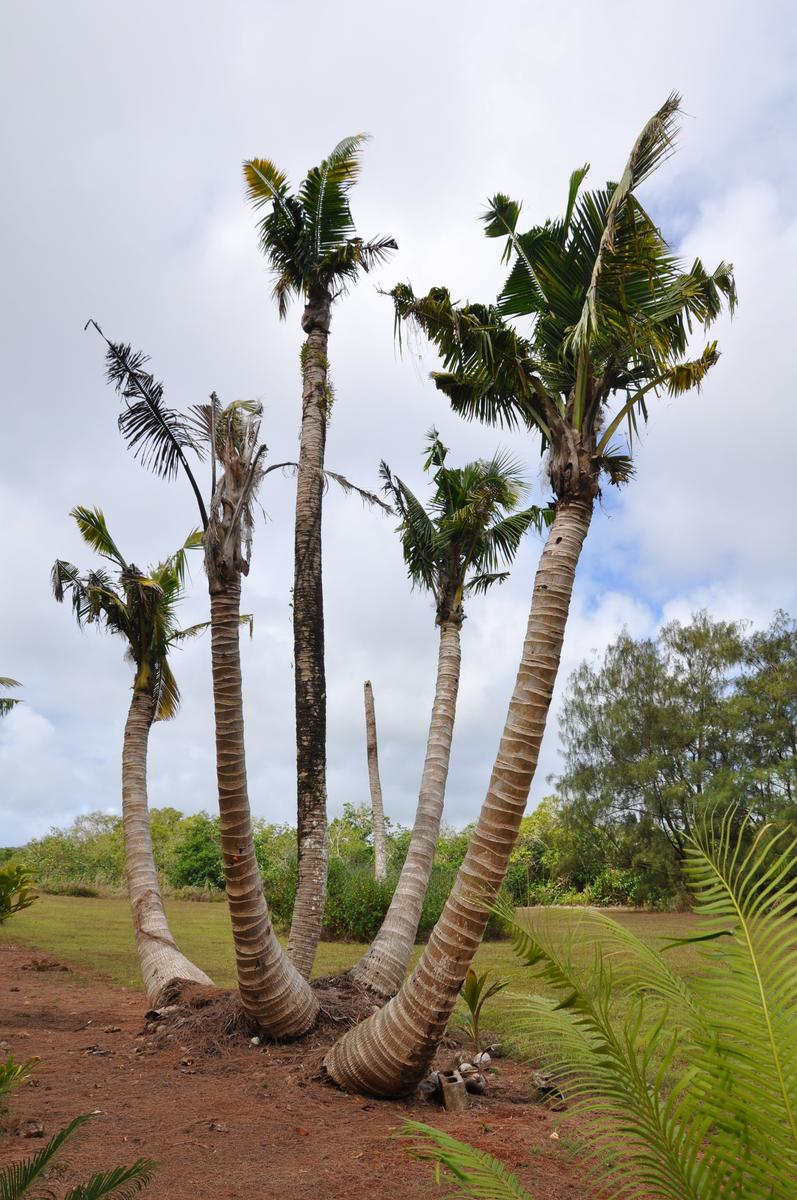
\includegraphics[width=0.8\linewidth]{images/dying_coconuts}
	\caption{Coconut palms severely attacked by coconut rhinoceros beetle.}
	\label{fig:dyingcoconuts}
\end{figure}

\begin{figure}[h]
	\centering
	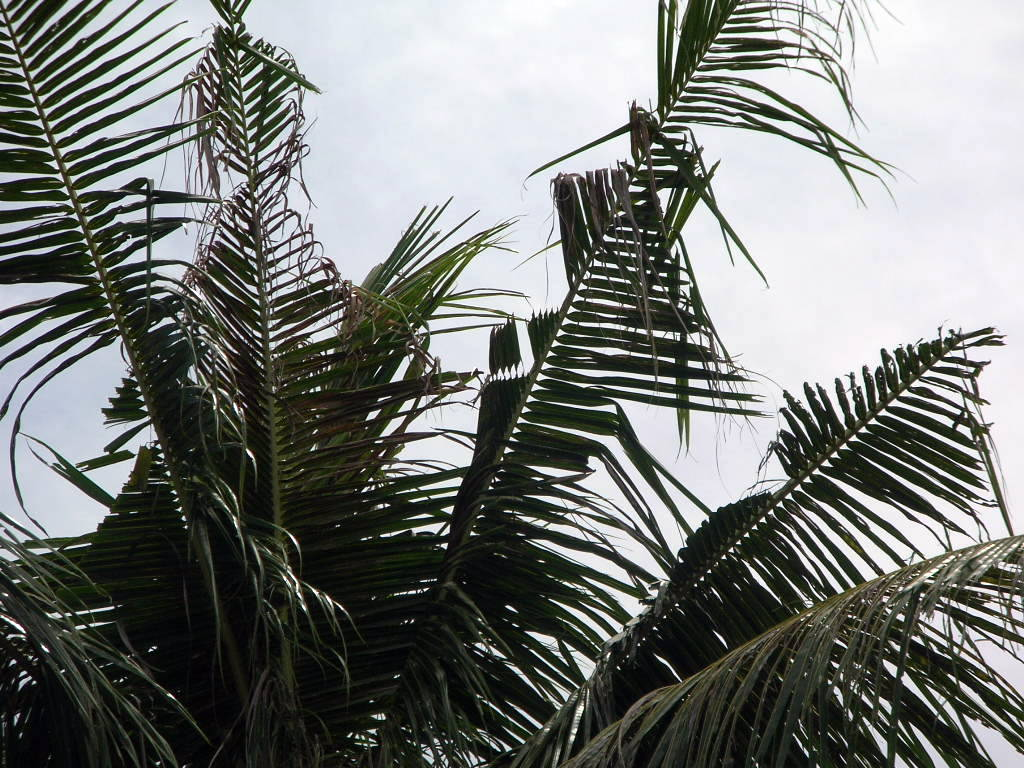
\includegraphics[width=0.7\linewidth]{images/vshaped-cuts}
	\caption{V-shaped cuts caused by adult CRB.}
	\label{fig:vshaped-cuts}
\end{figure}

\begin{figure}[h]
	\centering
	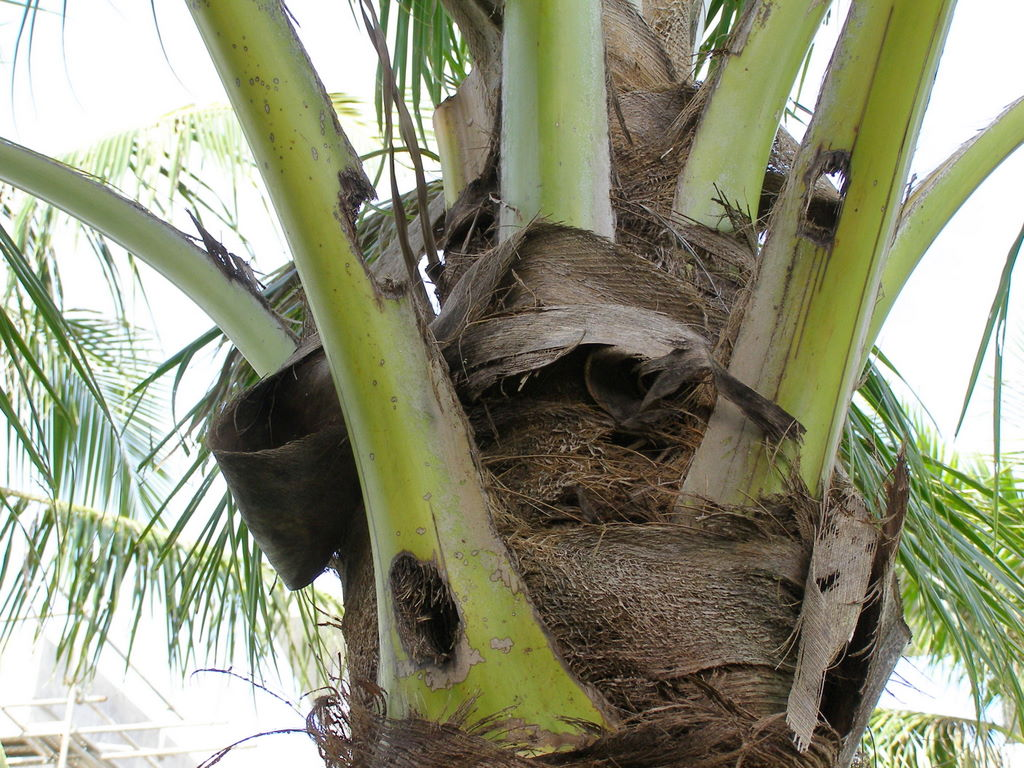
\includegraphics[width=0.7\linewidth]{images/bore-hole-through-petiole}
	\caption{CRB bore holes through petioles.}
	\label{fig:bore-hole-through-petiole}
\end{figure}

\begin{figure}[h]
	\centering
	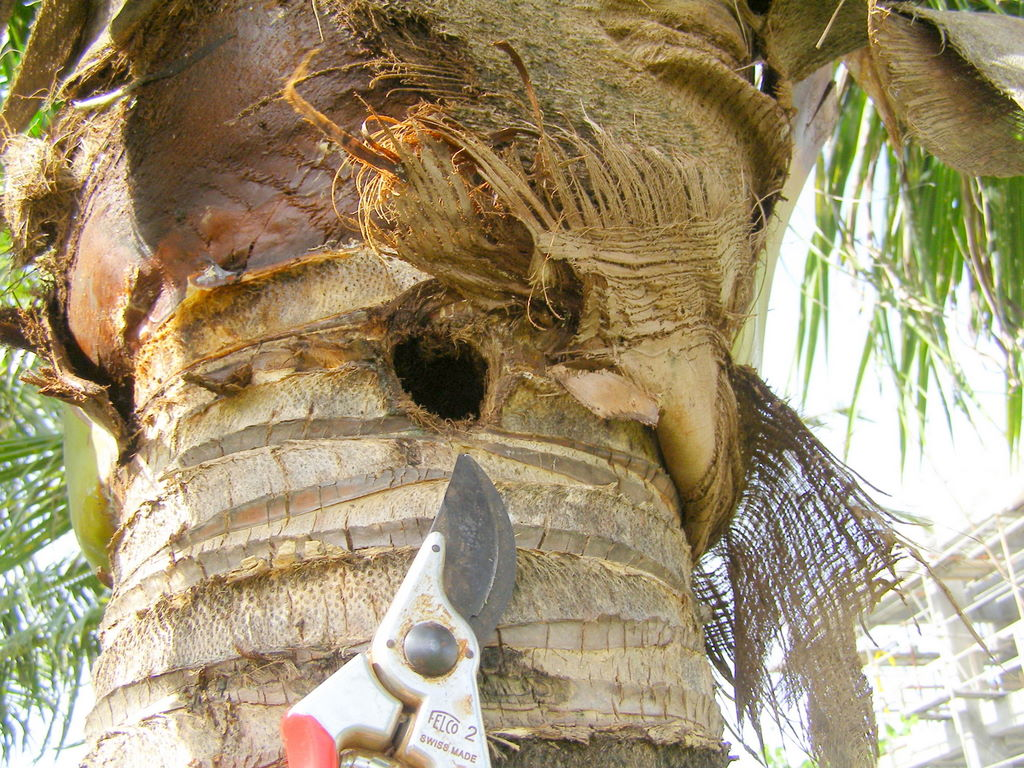
\includegraphics[width=0.7\linewidth]{images/bore-hole}
	\caption{CRB bore hole in stem made visible by removing petioles.}
	\label{fig:bore-hole}
\end{figure}

\subsection{Population dynamics}

With unlimited food and no control from natural enemies, CRB populations are capable of growing at a rate of about 3,250\% per generation. Devastating, uncontrolled outbreaks of CRB are often triggered by a tropical cyclone, massive land clearing or military activity which generates large amounts of dead and decaying vegetation over a large area. Within a few months, this plentiful food supply generates massive numbers of adults which bore into palm crowns. The high rate of attack results in high palm mortality. These dead palms quickly begin to rot and become ideal CRB breeding sites, generating even higher numbers of adults which bore into and kill even more palms. In the absence of natural enemies or introduced biological control agents, this self-sustaining feedback cycle may result in the loss of most palm trees on an island. 

An example of this positive feedback cycle occurred in Palau as a result of massive destruction of palms and other vegetation during the Second World War. Prior to the war, CRB was very rare in Palau but shortly afterwards about 50\% of coconut palms were killed by CRB throughout the archipelago, and some islands lost all of their palms.

Uncontrolled outbreaks of CRB-G are currently happening on Guam and some of the Solomon Islands.

\subsection{Geographic distribution}

Islands in the Pacific and Indian Oceans were invaded by CRB during two waves of movement (Fig. \ref{fig:crbdist}). The first wave started in 1909 when CRB was accidentally transported to from Sri Lanka to Samoa with shipment of rubber tree seedlings and it ended during the 1970s. All of the CRB range expansion during this period was south of the equator except for the invasion of the Ryuku Islands (Japan) starting in 1921 and invasion of the Palau Islands prior to 1943.

The second wave of CRB invasions started in 2007 with discovery of CRB on Guam, followed by invasion of Oahu (Hawaii), Port Morseby (Papua New Guinea), Guadalcanal, Savo and Malaita (Solomon Islands), and Rota (Commonwealth of the Northern Mariana Islands). Beetles in the second wave of invasions are genetically different from those in the first wave and these are being referred to as the Guam biotype or CRB-G for short.

\begin{figure}[h!]
	\centering
	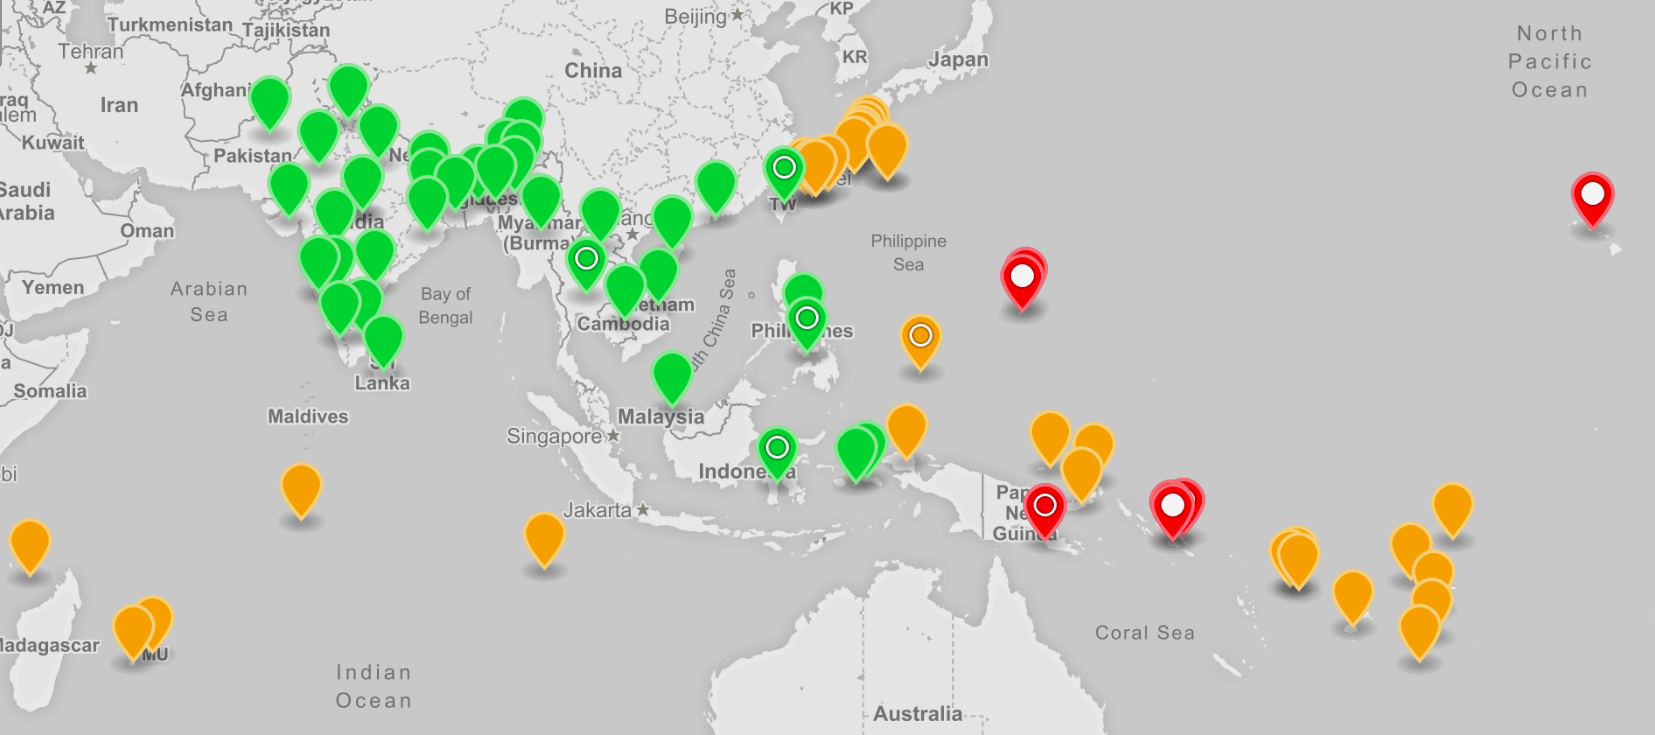
\includegraphics[width=\linewidth]{images/crb_dist}
	\caption{Screenshot of an online interactive web map showing the geographic distribution of the coconut rhinoceros beetle. Green markers: native range; Orange markers: first detected during the 20th century; Red markers first detected during the 21st century; Open circle: population includes CRB-G biotype; Filled circle: population is exclusively CRB-G biotype.}
	\label{fig:crbdist}
\end{figure}

\section{Control tactics}

\subsection{Eradication}

In theory, eradication of CRB from a newly invaded area can be attained by blocking invasion pathways coupled with finding and destroying all breeding sites. In practice, eradication has proven to be very difficult after initial establishment of a CRB population, despite early detection and rapid response. 

Only one of many eradication attempts has succeeded. This was accomplished on the tiny (36 km\textsuperscript{2}) Niuatoputapu Island (also known as Keppel Island), which lies between Samoa and Tonga. During a period spanning 1922 to 1930 all CRB breeding sites were located and destroyed.

\subsection{Sanitation}

Sanitation includes detection and destruction of active and potential CRB breeding sites.

\paragraph{Breeding site detection}

Local searches for breeding sites are usually initiated in response to visible damage to palms or capture of adults in pheromone traps. In Guam and Hawaii, dogs trained to sniff out CRB grubs have been deployed to assist human searchers. Recent research suggests that CRB adults fitted with miniature radio transmitters or harmonic radar tags may be a cost effective way of detecting cryptic breeding sites. The essential idea is that the radio transmitters and tags will accumulate at breeding sites where adults aggregate. These tags can then be detected by ground and/or aerial surveys using radio receivers or harmonic radar transceivers.

\paragraph{Removal of standing dead palms}
CRB adults are attracted to standing dead palm trees that have begun to rot from the crown. Females will lay their eggs in the rotting palm trunk and the developing larvae will feed on the decaying fibers near the top of the trunk, which starts to decompose in the center forming a protective tube for larval development. As the larvae increase in size and strength of their mandibles, they can penetrate further down the trunk leaving a column of frass and cut fibers for the early instars. Dead standing palms should be felled, cut into pieces and burnt or buried to remove potential breeding sites. In some situations, larvae may develop in the crown of live palms. This only occurs where there are large accumulations of organic matter in the frond bases. The organic matter should be removed where possible.

\paragraph{Disposal of dead felled palms}
Mature palm trees will fall after being weakened by fungal diseases (\textit{Ganoderma}), after strong winds during tropical cyclones or after the felling of senile palms prior to replanting. Dead palms on the ground should be cut up into manageable lengths or chipped prior to disposal by burning or deep burial. 

\paragraph{Covering of palm stumps}
Felled palms leave a stump which is suitable for development of larvae as it rots. In management of palm plantations in Asia, where a zero-burning policy is in operation, ground cover is planted shortly after felling to cover the debris and make it less attractive to the flying beetles. The legumes \textit{Mucuna} spp. and \textit{Pueraria javanica} are ground cover plants that are commonly used, as they will add nitrogen to the soil and cover the decaying trunks. 

\paragraph{Management of organic matter and compost}
Heaps  of  organic  matter,  particularly  palm  debris,  provide  excellent  food  material  for  development  of  CRB larvae. Any deep piles of organic material will be attractive to the egg laying females. Heaps of fronds or empty fruit bunches are particularly susceptible. Sawdust from sawmills that process palm timber is also a favorable resource for beetle development. General compost, farmyard manure and even organic garbage can provide sites for development of the larvae. The first step in reducing the threat of beetles emerging from composts is management of the organic matter. Palm debris should be spread among the palms to break down rapidly and release nutrients rather than being piled in heaps. Compost or farmyard manure should be turned regularly, and larvae removed, or pigs and chickens can assist by eating exposed larvae. In urban environments, organic material is often gathered during environmental clean-up and composted, but this may provide a centre for re-infestation of the locality. Compost can be sterilized or fumigated to kill larvae; however, this process is energy-demanding  and  expensive.  Sterile  compost  will  also  be  susceptible  to  re-invasion. Where  feasible,  compost heaps can be covered with netting to trap emerging beetles.

Burning CRB breeding material is the most dependable method for removing the food source for CRB grubs. In Hawaii CRB sanitation programs, breeding site material is being burned on-site using air-curtain burners and some is being trucked to a waste-to-energy electrical power generation plant. 

\subsection{Trapping}

CRB trapping can be used for different purposes including surveillance for early detection, monitoring growth and spread of a population over time, and for population suppression by mass trapping. In all cases, the trap needs to be attractive enough to draw in beetles from a distance strong and enough to contain them once they are captured. Olfactory and visual attractants can be used to increase trap catch. 

\paragraph{Artificial breeding sites} One of the first traps to be developed was the Hoyt trap made from a metal can set on top of a coconut trunk or wooden post (Fig. \ref{fig:hoyt-trap}). The can was capped with a length of coconut stem with a hole in the center large enough for a beetle to enter. The trap system was used extensively and functioned because it mimicked a standing, decaying coconut stem which is attractive to CRB adults. 

An artificial breeding site trap can easily be constructed simply by laying coconut log sections on the ground (Fig. \ref{fig:log-tap}). Trap catch can be enhanced by covering the logs with netting (see section on netting below) and providing a pheromone source.
\begin{figure}[h]
	\centering
	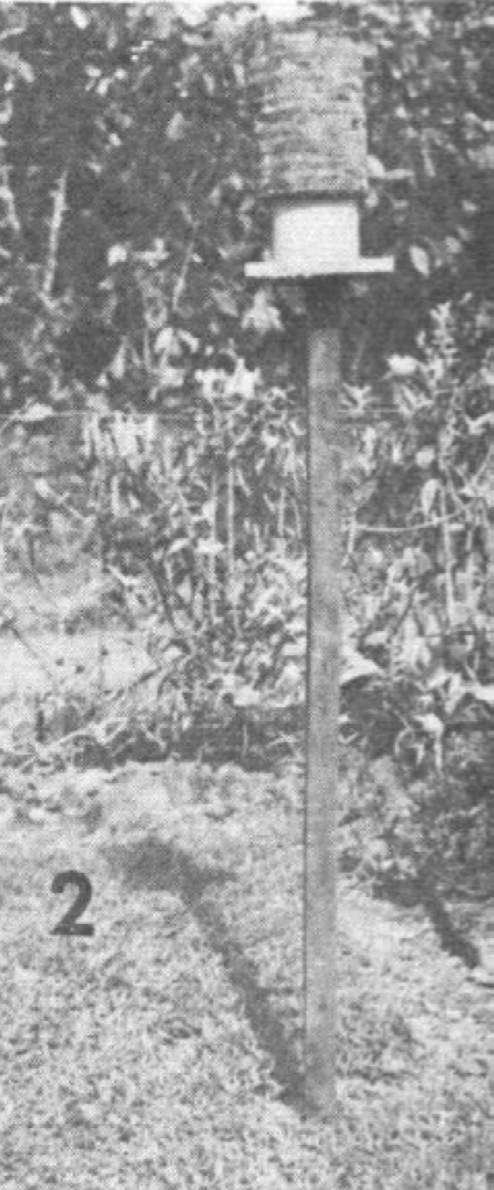
\includegraphics[width=0.7\linewidth]{images/hoyt-trap}
	\caption{A Hoyt trap for capturing CRB adults.}
	\label{fig:hoyt-trap}
\end{figure}

\begin{figure}[h]
	\centering
	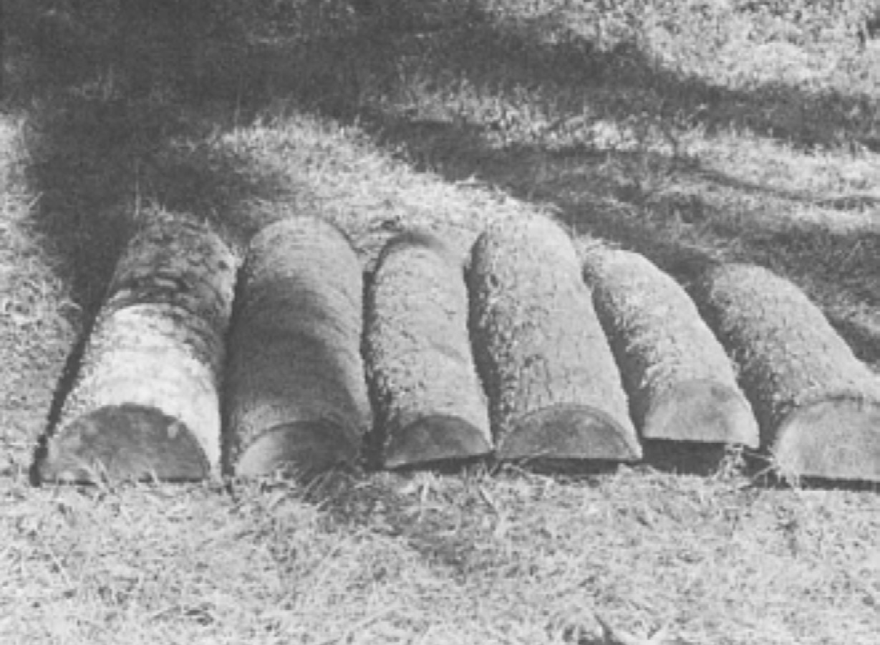
\includegraphics[width=0.7\linewidth]{images/log-tap}
	\caption{A log trap for capturing CRB adults.}
	\label{fig:log-tap}
\end{figure}

\paragraph{Pheromone traps} Design and utility of traps changed with the discovery of ethyl chrysanthemate as an attractant. This was rapidly superseded by ethyl-4-methyloctanoate (E4-MO) commonly referred to as oryctalure, the male-produced aggregation pheromone of CRB, which could be synthesized. E4-MO attracts both sexes, has been used for more than 30 years and is produced commercially by several companies. 

Pheromone traps for surveillance need to be robust, inexpensive, attractive to beetles, difficult to exit and simple to service. Simple bucket traps are used extensively for monitoring throughout the Pacific Islands and Southeast Asia (Fig. \ref{fig:spc-bucket}). Vaned bucket traps (Fig. \ref{fig:uog-bucket}) and panel traps (Fig. \ref{fig:panel-trap}) have been used in surveillance trapping in Guam and Hawaii where thousands of traps have been deployed to monitor of the spread of CRB populations and success of control activities.
\begin{figure}[h]
	\centering
	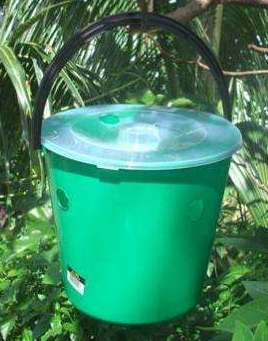
\includegraphics[width=0.7\linewidth]{images/spc-bucket}
	\caption{A bucket trap for capturing CRB adults. An oryctalure dispenser is hung from the lid, inside the bucket. Beetles enter through holes in the top and sides of the bucket.}
	\label{fig:spc-bucket}
\end{figure}

\begin{figure}[h]
	\centering
	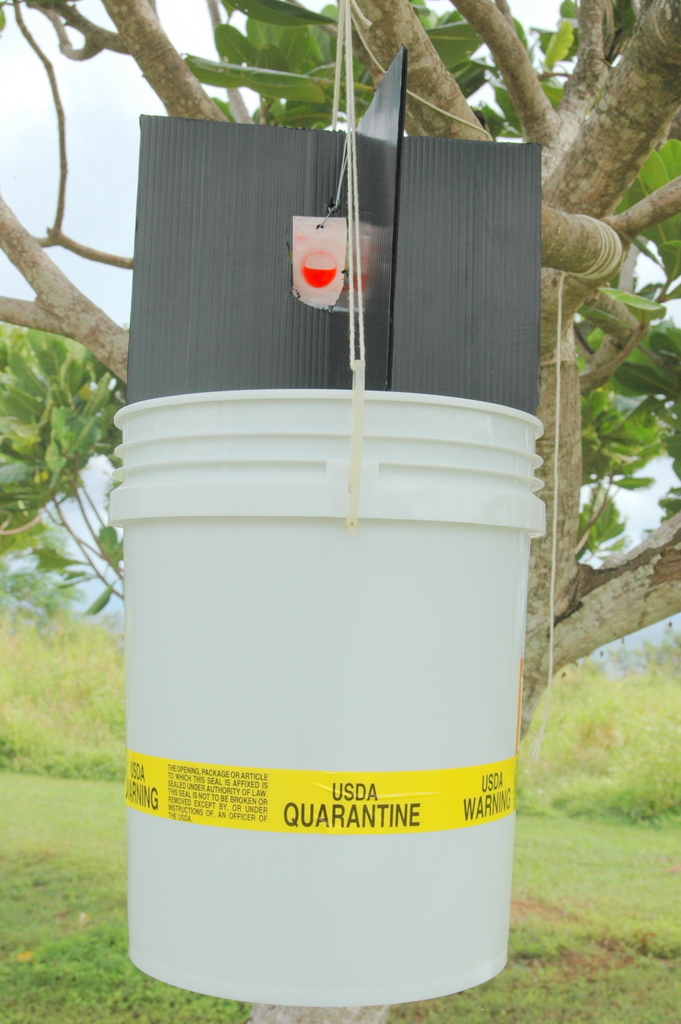
\includegraphics[width=0.7\linewidth]{images/uog-bucket}
	\caption{A vaned bucket trap for capturing CRB adults. An oryctalure dispenser is visible at the center of the vanes.}
	\label{fig:uog-bucket}
\end{figure}

\begin{figure}[h]
	\centering
	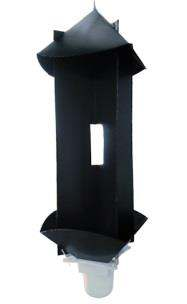
\includegraphics[width=0.7\linewidth]{images/panel-trap}
	\caption{A commercially manufactured panel trap for capturing CRB adults. An oryctalure dispenser is hung in the rectangular hole at the center of the vanes.}
	\label{fig:panel-trap}
\end{figure}

\paragraph{Efficacy of pheromone traps for population suppression} Trapping removes adults from the population and may contribute to pest and damage reduction. Bucket traps baited with pheromone have been reported to reduce CRB populations in Malaysia and the related \textit{O. monoceros} in West Africa. 

However, efficacy of pheromone traps for populations of CRB-G is in question.
Mass trapping was performed on Guam shortly after detection of CRB in the Tumon Bay hotel area in 2007. There was no indication of population suppression and trapping did not reduce damage to palms with the mass trapping areas. During 2010, the trap catch rate in Tumon Bay was only 0.006 beetles per trap day, but CRB damage was visible in 100\% of coconut palms. In contrast, a similar mass trapping program in Samoa trapped 0.150 per trap-day, 25 times the Guam trap-catch rate, but the proportion of damaged coconut palms was only 30\%. Note that the Guam population is the CRB-G biotype and the Samoan population is the CRB-S biotype. 

Three possible explanations have been suggested to account for these observations:
\begin{enumerate}
\item Traps baited with oryctalure are more attractive to CRB-S than CRB-G.
\item CRB-G individuals do far more damage than CRB-S individuals.
\item At very high population levels and trap densities there is so much pheromone in the air that beetles cannot navigate to pheromone sources.
\end{enumerate}

In mark-release-recapture experiments on Guam only 64 of 567 (11\%) of marked beetles where recaptured in a grid of traps baited with oryctalure, indicating that oryctalure is not highly attractive to CRB-G biotype. Unfortunately, there are no comparative data for the CRB-S biotype.  

\paragraph{Netting} Tekken, a gill net used by Chamorro fishermen on Guam, has proven to be an effective trapping tool for coconut rhinoceros beetles. Beetles are captured when a strand of the netting falls into the gap behind a beetle's pronotum, in the same way that fish are caught when a strand falls into a gill slit (Fig. \ref*{fig:tekken-beetle}). In Guam, heaps of organic waste are covered with tekken which traps outgoing beetles emerging from the pile and incoming beetles attracted to the heaps for mating and oviposition (Fig. \ref{fig:tekken-pile}). 

Cheap and simple pheromone traps can be made by attaching pieces of tekken to fences and placing an oryctalure dispenser at the center of each piece (Fig. \ref{fig:defence-trap}). 

%\begin{figure}[h]
%	\centering
%	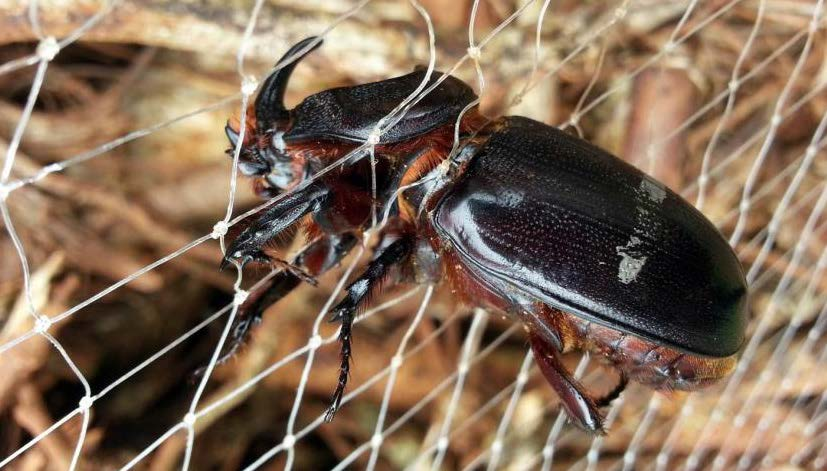
\includegraphics[width=\linewidth]{images/tekken-beetle}
%	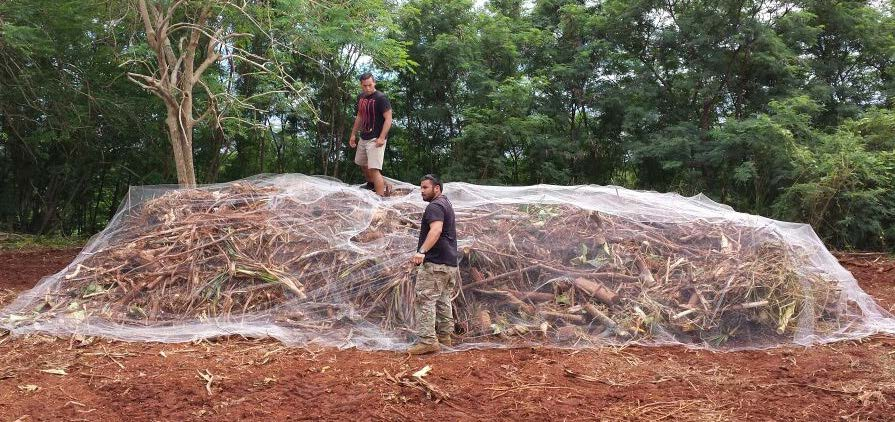
\includegraphics[width=\linewidth]{images/tekken-pile}
%	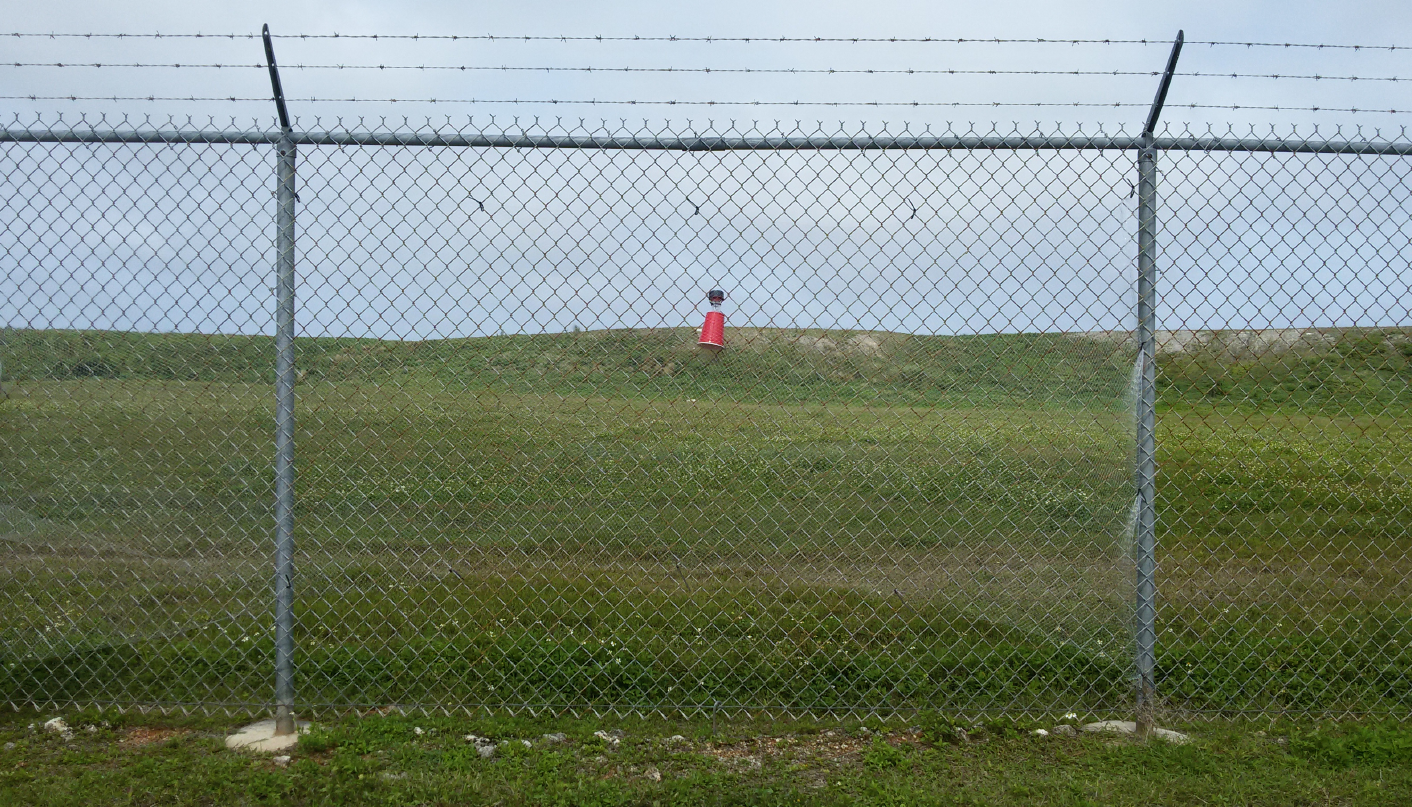
\includegraphics[width=\linewidth]{images/defence-trap}
%	\caption{Tekken.}
%	\label{fig:tekken-beetle}
%\end{figure}

\begin{figure}[h]
	\centering
	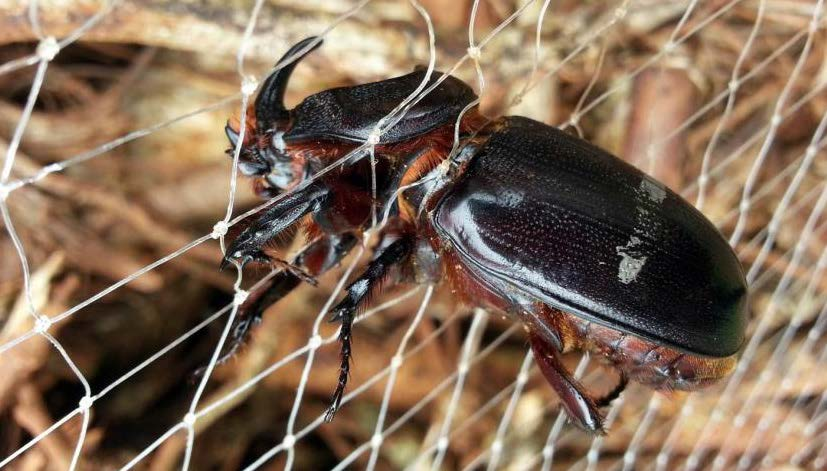
\includegraphics[width=0.7\linewidth]{images/tekken-beetle}
	\caption{A CRB adult captured by tekken fish netting.}
	\label{fig:tekken-beetle}
\end{figure}

\begin{figure}[h]
	\centering
	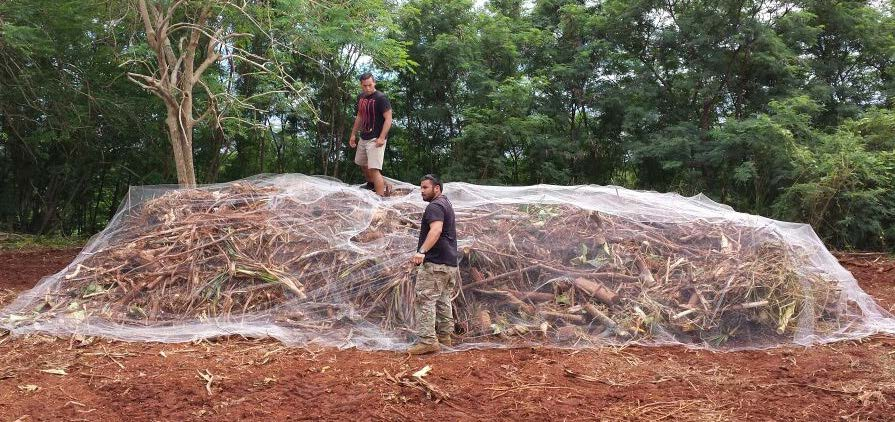
\includegraphics[width=0.7\linewidth]{images/tekken-pile}
	\caption{Tekken fish netting used to cover a pile of greenwaste.}
	\label{fig:tekken-pile}
\end{figure}

\begin{figure}[h]
	\centering
	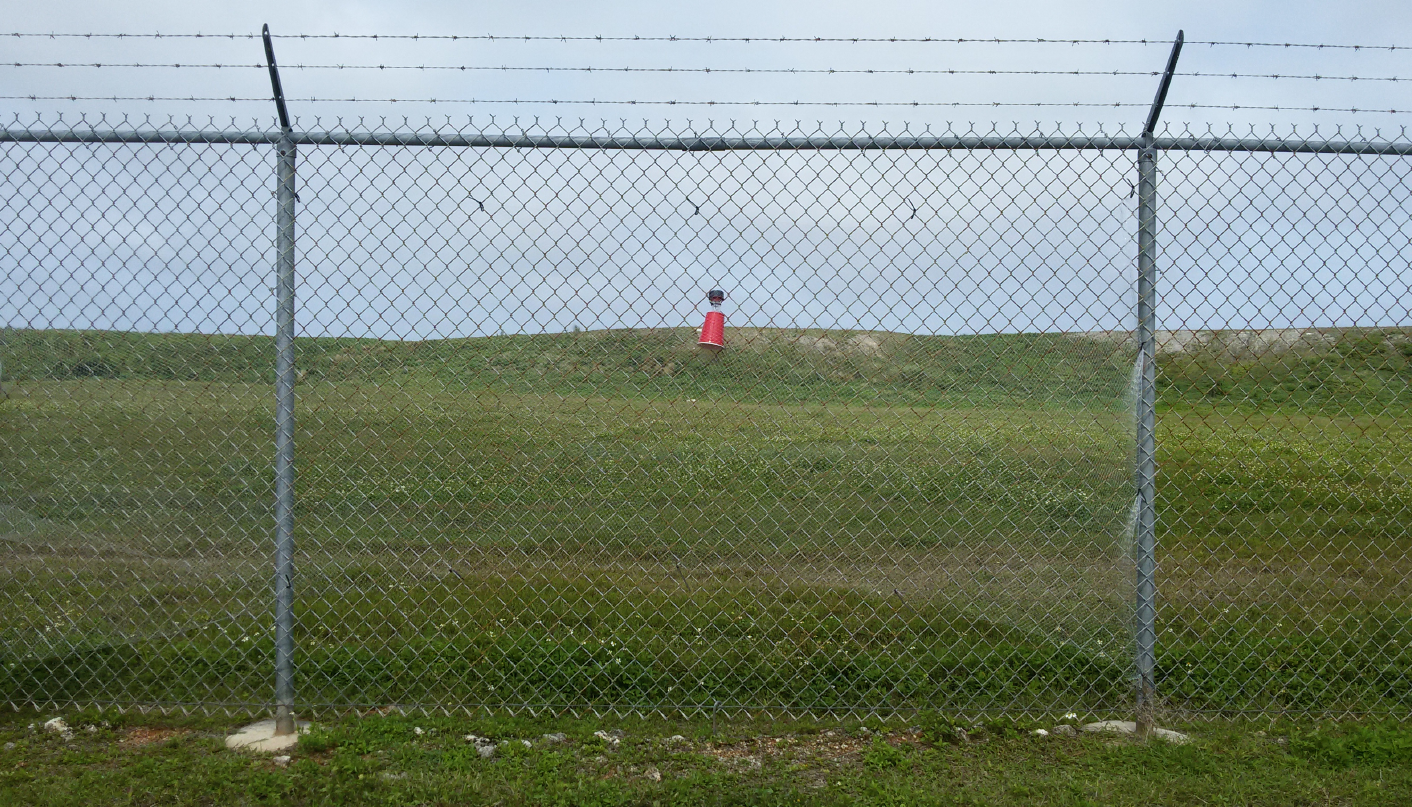
\includegraphics[width=0.7\linewidth]{images/defence-trap}
	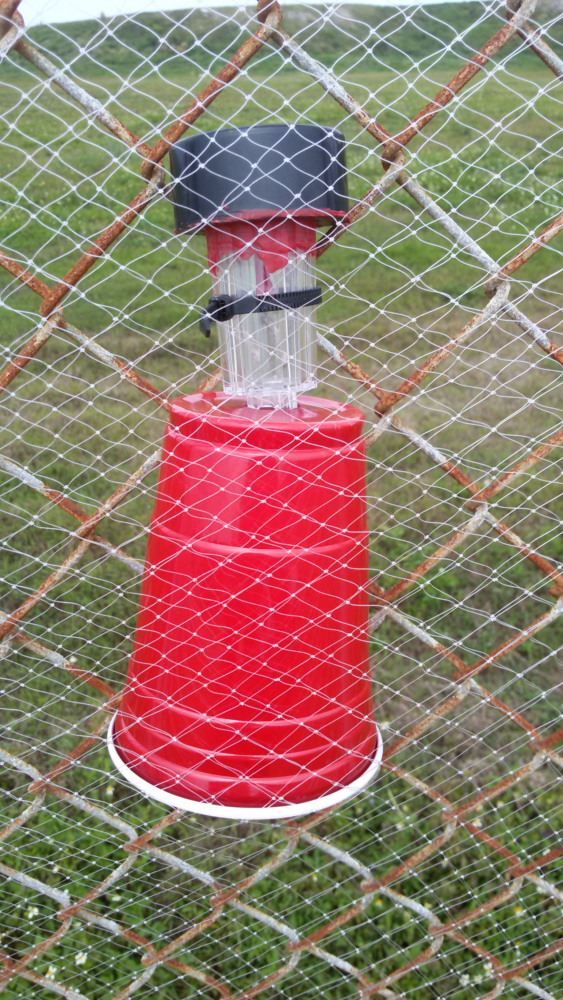
\includegraphics[width=0.23\linewidth]{images/defence-trap-lure}	
	\caption{A Defence trap for trapping CRB adults. Constructed by attaching a piece of tekken fish netting to a fence and hanging an oryctalure dispenser near the center. The dispenser shone here has the oryctalure covered by an upturned cup to protect it from the sun and wind. Above the cup is an solar powered ultraviolet light emitting diode which increases trap catch by about 3X.}
	\label{fig:defence-trap}
\end{figure}

\subsection{Chemical control}
Chemical control of CRB is difficult because all life stages live in protected habitats: grubs and adults may found inside dead logs or buried in or under heaps of decaying vegetation and adults may be found boring into palm crowns only briefly, for a few days during feeding bouts. 

Federal and state pesticide regulations should be checked before planning any chemical control activities.

\paragraph{Foliar application}
Foliar insecticide application is aimed at preventing damage or mortality of palms caused by adults. The pyrethroid, cypermethrin has been used to successfully protect coconut palms and oil palms. A high enough volume should be applied so that the pesticide runs down the midrib and pools at the base of the petiole where it meets the crownshaft. This is the location at which CRB adults initiate bore holes. Foliar sprays may be applied by hydraulic sprayers or by pesticide applicator drones.  

\paragraph{Trunk injection}
Trunk injections of systemic insecticides have been applied to oil palms and coconut palms with variable success.

\paragraph{Treatment of breeding sites}
Cypermethrin applied as a drench controls all life stages in heaps of loose breeding site material, but may not kill adults and grubs living inside logs.

\subsection{Biological control}

Biological control is the use of natural enemies (predators, pathogens, parasites) to suppress pest populations. In its native range, CRB is attacked by a community of co-evolved natural enemies, including pathogenic viruses and fungi, predatory carabid and elaterid beetles  and  parasitic  \textit{Scolia}  wasps.  The  relative  impact  of  each  natural  enemy  species  within  this  native community is poorly known, with additional control strategies often needed to complement biological control in coconut and oil palm plantations.

When CRB-S invaded the Pacific, it was the focus of a substantial biological control  program.  The  aim was to find one or more natural enemies in the native range that could be introduced to the invaded range to  suppress  CRB-S  populations.  This  process  is  known  as  classical  biological  control. Among many natural enemies introduced to the Pacific, very few predators or parasites established. Incidental predation by pigs and chickens on CRB larvae may assist with control of this pest and can be useful for control of larvae in household or community waste piles. Local species of generalist arthropod predators (centipedes, beetles, ants) may feed on CRB larvae; however, there is 
little evidence that this contributes significantly to CRB control. 

Only one pathogen provided significant control of CRB-S: the \textit{Oryctes rhinoceros} nudivirus (OrNV) discovered in Malaysia by Alois M. Huger in 1963. This virus infects CRB-S larvae and adults, causing death after 6–30 days. Infected adults are weakened prior to death so that they stop feeding, their mobility is reduced and females stop laying fertile eggs. Once established in countries invaded by CRB-S, the virus significant reduced CRB populations and the damage they caused. 

Another approach to biological control for CRB was to create a biopesticide from a known pathogen. CRB adults and larvae can be infected by the fungus \textit{Metarhizium majus} (formerly \textit{M. anisopliae} var. \textit{majus}). This fungus has been developed into 
a biopesticide that can be applied to CRB breeding sites in both the native and invaded range. 

The recent invasion of CRB-G has changed CRB management wherever it is found. CRB-G is not susceptible to strains of OrNV introduced originally to control CRB-S in the Pacific. A new biological control effort is underway in order to identify strains of OrNV from CRB’s native range that are effective against CRB-G. Until an effective OrNV strain is discovered, biopesticides containing \textit{M. majus} are the only option for biological control of CRB-G.

In some jurisdictions, biological control agents are regulated as pesticides. For example, the U.S. Environmental Protection Agency regulates OrNV and \textit{M. majus} as pesticides. Federal and state pesticide regulations should be checked before using biological control agents for CRB. 

\subsection{Damage surveys}

A standardized method has been developed for quantifying CRB damage (for details see Jackson et. al 2020). This method uses a five-level scale is illustrated in the following figures (Figs \ref{fig:damage0}, \ref{fig:damage1}, \ref{fig:damage2}, \ref{fig:damage3}, \ref{fig:damage4}). 

This method can be applied by direct visual observation or by scoring palms appearing in images. Research is underway to develop automated detection and mapping of CRB damage by applying computer vision techniques to images recorded during ground-based and aerial drone surveys. 

\begin{figure}[p]
	\centering
	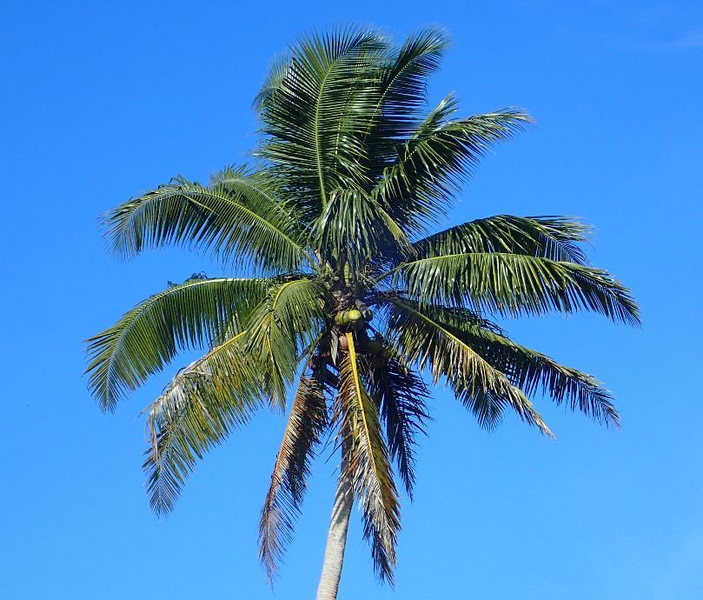
\includegraphics[width=.8\linewidth]{images/j5index0.resized.png}
	\caption{\textbf{Damage index 0}; Zero damage; No CRB damage visible}
	\label{fig:damage0}
\end{figure}

\begin{figure}[p]
	\centering
	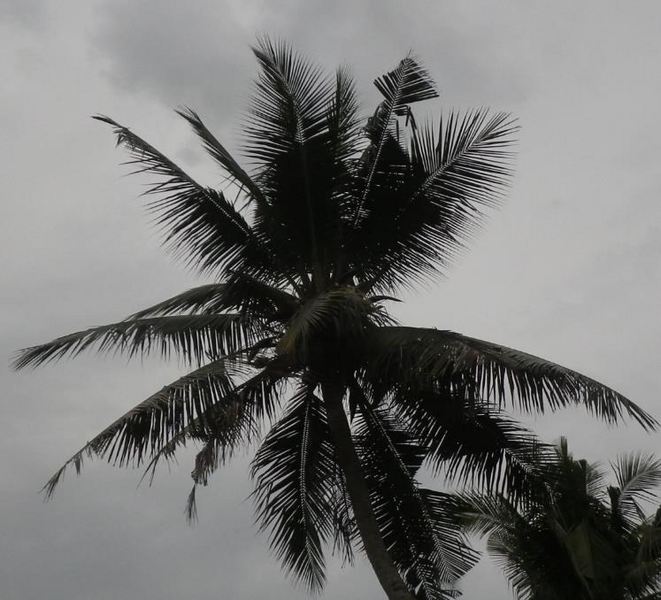
\includegraphics[width=.8\linewidth]{images/j5index1.resized.png}
	\caption{\textbf{Damage index 1}; Light damage; Notching or tip damage; less than less than 20\% foliar loss}
	\label{fig:damage1}
\end{figure}

\begin{figure}[p]
	\centering
	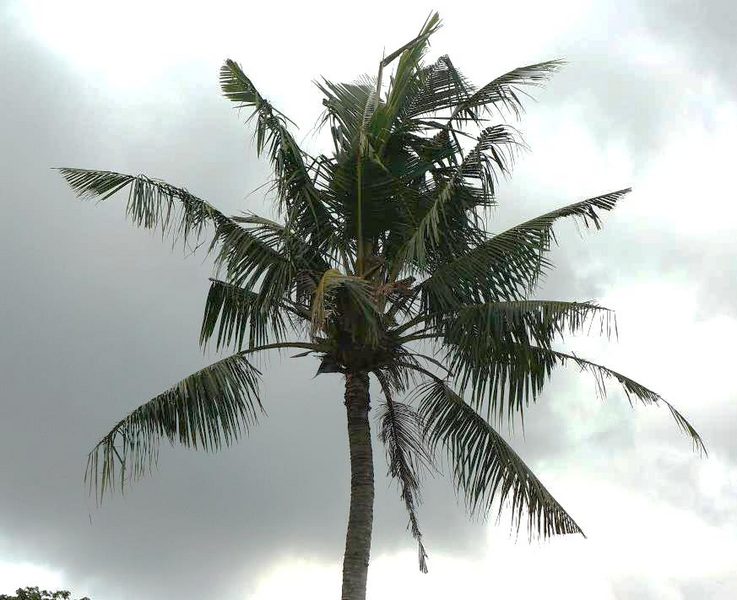
\includegraphics[width=.8\linewidth]{images/j5index2.resized.png}
	\caption{\textbf{Damage index 2}; Medium damage; Multiple fronds damaged; Notching and breakage; 20\% to 50\% foliar loss}
	\label{fig:damage2}
\end{figure}

\begin{figure}[p]
	\centering
	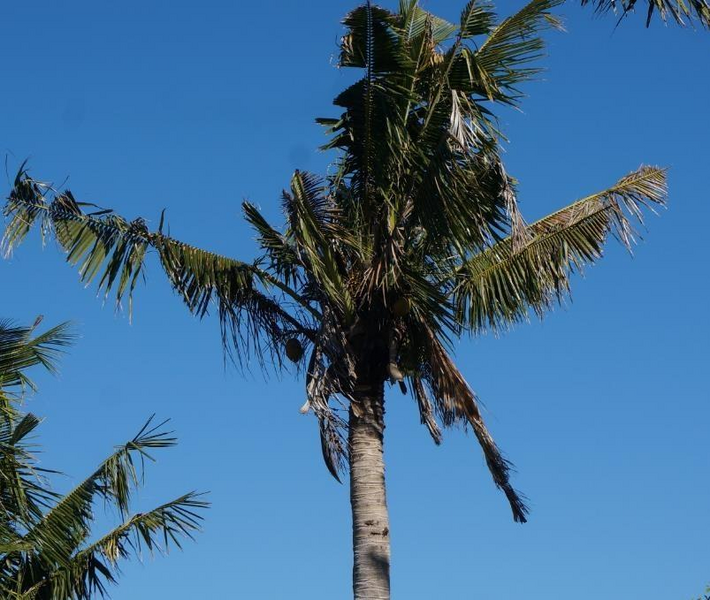
\includegraphics[width=.8\linewidth]{images/j5index3.resized.png}
	\caption{\textbf{Damage index 3}; High damage; greater than 50\% foliar loss}
	\label{fig:damage3}
\end{figure}

\begin{figure}[p]
	\centering
	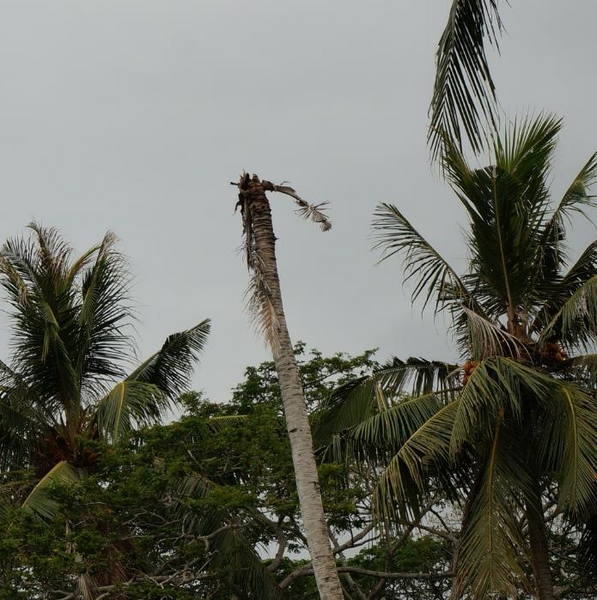
\includegraphics[width=.8\linewidth]{images/j5index4.resized.png}
	\caption{\textbf{Damage index 4}: Dead or moribund; Meristem destroyed}
	\label{fig:damage4}
\end{figure}

\newpage
\subsection{Integrated pest management}

Integrated pest management (IPM), is a broad-based approach that integrates practices for economic control of  pests.  The  Food and Agriculture Organization of the United Nations   IPM  as  “The careful consideration of all available pest control techniques and subsequent integration of appropriate measures that discourage the development of pest populations. It combines biological, chemical, physical and crop specific (cultural) management strategies and practices to grow healthy crops and minimize the use of pesticides, reducing or minimizing risks posed by pesticides to human health and the environment for sustainable pest management.”

IPM for management of CRB and includes combination of the tactics described above. 

For coconut palms planted for subsistence, ornamental purposes, or in commercial plantations, IPM for CRB involves: 
\begin{enumerate}
	\item monitoring of palm damage to detect localized CRB outbreaks and to check that control is successful
	\item biological control with OrNV (in the invaded and native range) and other co-evolved natural enemies (in the native range only)
	\item sanitation to remove organic waste, dead palms and  other  potential  breeding  sites
\end{enumerate}

Sanitation  is  an  essential  component  of  IPM  for  CRB  that  complements biological control. Localized CRB outbreaks will occur when breeding sites are left uncontrolled, especially after cyclones and tropical storms, when palms are often toppled by high winds and large amounts of green waste is created. Historically, outbreaks of CRB often follow cyclone damage or large scale land clearing. Larvae will develop in the decaying fronds, the trunk and even the roots of the felled palms and also in many other forms of decaying vegetation. 

Some additional options may be incorporated into IPM programmes for coconut, particularly for commercial plantations or ornamental palms. These more costly options include pheromone traps to monitor adult beetle activity and complement it with visual surveys of palm damage. Occasionally, trap catches may be high enough to  contribute  to  population  suppression  in  coconut  plantations,  but  this  strategy  is  more relevant to oil palm (discussed below). If a recent invasion of CRB is targeted for eradication, insecticides may  be  necessary  for  success.

For higher value crops, particularly oil palm, the same components are needed as for coconut: monitoring, biological control; and sanitation. More costly IPM components are recommended for oil palm because the crop’s financial value makes greater investment in control worthwhile. Thus, IPM for CRB in oil palm involves: 
\begin{enumerate}
	\item monitoring of beetle activity with pheromone traps and palm damage particularly for young palms
	\item biological control with OrNV (invaded and native range) and other natural enemies (native range) plus application of \textit{M. majus} as a biopesticide to breeding sites that cannot be removed
	\item sanitation to remove organic waste, particularly during plantation renewal when large amounts of waste is generated
	\item insecticide treatments for young palms that are most sensitive to CRB damage.
\end{enumerate} 

Note that pollinators of oil palm are vulnerable to insecticides, so applications should be scheduled carefully to avoid flowering. When oil palm plantations are renewed, complete clean-up of the organic waste is challenging. In CRB’s native range, an additional strategy is to break up and spread the waste as a thin layer, then plant a fast-growing cover crop, often a legume, over the waste matter. 

\newpage
\section*{References}

\paragraph{Bedford, Geoffrey O. 1980.} Biology, ecology, and control of palm rhinoceros beetles. Annual Review of Entomology 25 (1980): 309–39.
Available online at \url{https://tinyurl.com/yh79wmwc}

\paragraph{Gressitt, J. Linsley 1953.} The coconut rhinoceros beetle (\textit{Oryctes rhinoceros}) with particular reference to the Palau Islands. Bernice P. Bishop Museum. Bulletin 212. 
Available online at \url{https://tinyurl.com/npsab5d4}

\paragraph{Jackson, Trevor, Sean Marshall, Sarah Mansfield and Fereti Atumurirava 2020.} Coconut rhinoceros beetle (\textit{Oryctes rhinoceros}): A manual for control and management of the pest in Pacific Island countries and territories. Pacific Community (SPC). 
Available online at \url{https://tinyurl.com/yxk4u27j} 

\paragraph{Marshall, Sean D. G., Aubrey Moore, Maclean Vaqalo, Alasdair Noble, and Trevor A. Jackson 2017.} A new haplotype of the coconut rhinoceros beetle, \textit{Oryctes rhinoceros}, has escaped biological control by \textit{Oryctes rhinoceros} nudivirus and is invading Pacific Islands. Journal of Invertebrate Pathology, 149, 127-134.
Available online at \url{https://tinyurl.com/mtpp29da}

\paragraph{Pallipparambil, Godshen R. 2015.} New Pest Response Guidelines: \textit{Oryctes rhinoceros} (L.) Coleoptera: Scarabaeidae, Coconut rhinoceros beetle. U.S. Department of Agriculture, Animal Plant Health Inspection Service, Plant Protection and Quarantine.
Available online at \url{https://tinyurl.com/mpdmvfpt}

%\nocite{jackson_coconut_2020}
%
%
%\printbibliography

\end{document}
